\documentclass[11pt,a4paper]{article}
\usepackage[margin=24mm]{geometry}
\usepackage{amsmath,amssymb,bm}
\usepackage{tikz}
\usetikzlibrary{arrows.meta,calc}
\usepackage{microtype}
\usepackage[hidelinks]{hyperref}
\usepackage{caption}
\setlength{\parindent}{0pt}
\setlength{\parskip}{6pt}
\newcommand{\vect}[1]{\boldsymbol{#1}}
\newcommand{\ndc}{\mathrm{ndc}}
\newcommand{\clip}{\mathrm{clip}}
\numberwithin{equation}{section}
\begin{document}
\appendix
\section{Projection matrices}
This appendix derives the mappings from three-dimensional scene points to a two-dimensional display. Orthogonal projection is introduced first, followed by perspective projection for a centred eye and off-axis projection for an eye displaced relative to a fixed screen. The distinction between projection onto the physical screen and the graphics pipeline's clipping transformation is maintained throughout.

We use column vectors and a right-handed coordinate system with $x$ pointing right, $y$ pointing up, and the viewing direction along negative $z$. Initially, the eye is at the origin and the physical screen is the plane $z=-d$, where $d>0$. Its horizontal and vertical bounds are $[L,R]$ and $[B,T]$. A point is denoted $\vect p=(x,y,z)^{\mathsf T}$ and its homogeneous representation is $\widetilde{\vect p}=(x,y,z,1)^{\mathsf T}$. When clipping is introduced, the near and far planes are $z=-n$ and $z=-f$, with $0<n<f$. We use the OpenGL depth convention $z_{\ndc}\in[-1,1]$.

\subsection{Orthogonal projection}
Let a plane contain a point $\vect s$ and have unit normal $\vect k$. Orthogonal projection removes the component of $\vect p-\vect s$ parallel to $\vect k$:
\begin{equation}
\pi_{\perp}(\vect p)=\vect p-\vect k\bigl[\vect k^{\mathsf T}(\vect p-\vect s)\bigr]
=(I-\vect k\vect k^{\mathsf T})\vect p+\vect k\vect k^{\mathsf T}\vect s.
\end{equation}
The linear part $Q=I-\vect k\vect k^{\mathsf T}$ satisfies $Q^2=Q$ and $Q^{\mathsf T}=Q$: it is an orthogonal projection matrix onto the plane parallel to the screen through the origin. Projection onto an offset screen is affine, represented in homogeneous coordinates by
\begin{equation}
\Pi_{\perp}=\begin{pmatrix}I-\vect k\vect k^{\mathsf T}&\vect k\vect k^{\mathsf T}\vect s\\\vect 0^{\mathsf T}&1\end{pmatrix}.
\end{equation}
For the screen $z=-d$, choose $\vect k=(0,0,1)^{\mathsf T}$ and $\vect s=(0,0,-d)^{\mathsf T}$. Then
\begin{equation}
\Pi_{\perp}=\begin{pmatrix}1&0&0&0\\0&1&0&0\\0&0&0&-d\\0&0&0&1\end{pmatrix},
\qquad \pi_{\perp}(x,y,z)=(x,y,-d).
\end{equation}
Thus every point moves along a line perpendicular to the screen; apparent size does not depend on depth. The screen coordinates become
\begin{equation}
x_{\ndc}=\frac{2x-(R+L)}{R-L},\qquad
y_{\ndc}=\frac{2y-(T+B)}{T-B}.
\end{equation}
For rendering, depth is retained for visibility testing rather than collapsed onto the screen. Requiring $z=-n\mapsto-1$ and $z=-f\mapsto1$ gives the orthographic clipping matrix
\begin{equation}
P_{\mathrm{ortho}}=\begin{pmatrix}
\frac{2}{R-L}&0&0&-\frac{R+L}{R-L}\\
0&\frac{2}{T-B}&0&-\frac{T+B}{T-B}\\
0&0&-\frac{2}{f-n}&-\frac{f+n}{f-n}\\
0&0&0&1
\end{pmatrix}.
\end{equation}
Unlike $\Pi_{\perp}$, this matrix does not flatten space and is not generally idempotent. The term \emph{projection matrix} here refers to its role in rendering; the final image uses its first two coordinates.

\newpage
\subsection{Perspective projection onto the screen}
Perspective projection assigns a scene point to the intersection of the screen with the line joining that point to the eye. The screen lies between the eye and points behind the display, so it acts as a window onto the virtual scene, as illustrated in Figure~\ref{fig:perspective}.

\begin{figure}[h!]
\centering
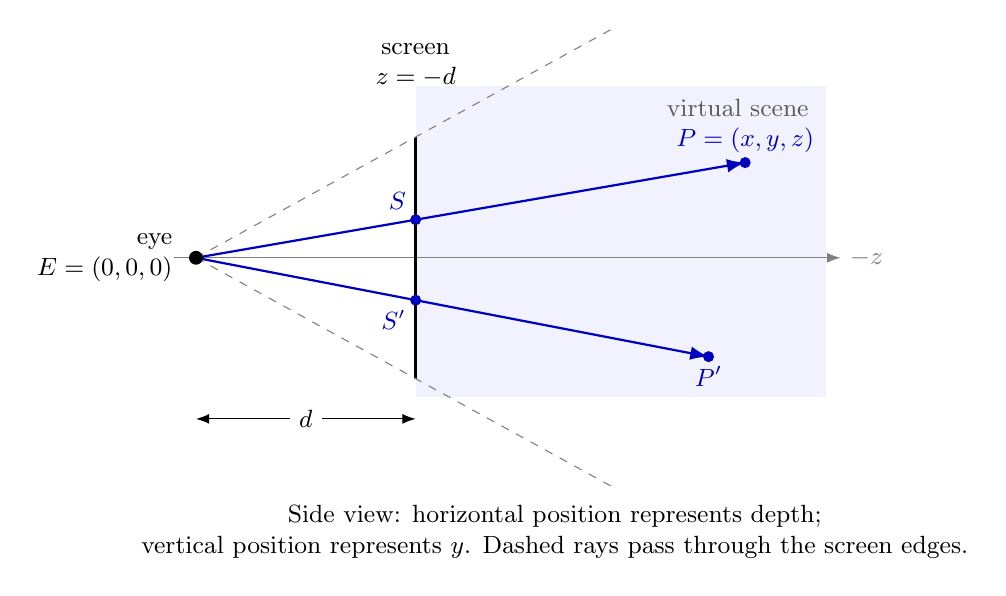
\begin{tikzpicture}[x=0.93cm,y=0.93cm,>=Latex,font=\small]
\fill[blue!5] (3,-1.9) rectangle (8.6,2.35);
\node[anchor=north east,text=black!65] at (8.5,2.3) {virtual scene};
\draw[->,gray] (-.3,0)--(8.8,0) node[right] {$-z$};
\draw[very thick] (3,-1.65)--(3,1.65);
\node[above,align=center] at (3,2.2) {screen\\$z=-d$};
\draw[blue!75!black,thick,->] (0,0)--(7.5,1.3);
\draw[blue!75!black,thick,->] (0,0)--(7,-1.35);
\draw[dashed,gray] (0,0)--(5.7,3.135);
\draw[dashed,gray] (0,0)--(5.7,-3.135);
\fill (0,0) circle (2.5pt) node[left=5pt,align=right] {eye\\$E=(0,0,0)$};
\fill[blue!75!black] (3,.52) circle (2pt) node[above left] {$S$};
\fill[blue!75!black] (7.5,1.3) circle (2pt) node[above] {$P=(x,y,z)$};
\fill[blue!75!black] (3,-.579) circle (2pt) node[below left] {$S'$};
\fill[blue!75!black] (7,-1.35) circle (2pt) node[below] {$P'$};
\draw[<->] (0,-2.2)--(3,-2.2) node[midway,fill=white] {$d$};
\node[below,align=center] at (4.9,-3.25) {Side view: horizontal position represents depth;\\vertical position represents $y$. Dashed rays pass through the screen edges.};
\end{tikzpicture}
\caption{Centred perspective geometry. Rays from the eye pass through screen points $S,S'$ and continue to scene points $P,P'$. The construction in the horizontal cross-section is identical.}
\label{fig:perspective}
\end{figure}

A ray from the origin through $\vect p$ is $\vect r(\lambda)=\lambda\vect p$. Its intersection with $z=-d$ satisfies $\lambda z=-d$. Therefore, for $z\ne0$,
\begin{equation}\label{eq:screen}
\lambda=-\frac d z,\qquad
\pi_{\mathrm{persp}}(x,y,z)=\left(-\frac{dx}{z},-\frac{dy}{z},-d\right).
\end{equation}
For a point beyond the screen, $z<-d$, we have $0<\lambda<1$, so the intersection lies between the eye and the point. Points between the eye and screen can also be projected, with $\lambda>1$. Only intersections within the screen rectangle are displayed.

The division by $z$ makes this mapping nonlinear in Cartesian coordinates. Homogeneous coordinates encode it as a matrix multiplication followed by division by the resulting fourth coordinate:
\begin{equation}
H_d=\begin{pmatrix}d&0&0&0\\0&d&0&0\\0&0&d&0\\0&0&-1&0\end{pmatrix},
\qquad H_d\widetilde{\vect p}=(dx,dy,dz,-z)^{\mathsf T}.
\end{equation}
Dividing the first three components by $w=-z$ recovers~\eqref{eq:screen}. This singular matrix describes actual projection onto the screen. The rendering matrix derived next preserves depth instead.

\newpage
\subsection{The centred perspective matrix and its parameters}
Assume that the eye lies on the perpendicular through the centre of a screen of width $W$ and height $H$. Then $L=-W/2$, $R=W/2$, $B=-H/2$, and $T=H/2$. Similar triangles give the horizontal and vertical fields of view
\begin{equation}
\theta_x=2\arctan\frac{W}{2d},\qquad
\theta_y=2\arctan\frac{H}{2d}.
\end{equation}
Let $a=W/H$ and $q=\cot(\theta_y/2)=2d/H$. Normalising the screen coordinates in~\eqref{eq:screen} gives
\begin{equation}
x_{\ndc}=-\frac{2dx}{Wz}=-\frac{q}{a}\frac{x}{z},\qquad
y_{\ndc}=-\frac{2dy}{Hz}=-q\frac{y}{z}.
\end{equation}
Thus $w_{\clip}=-z$, $x_{\clip}=(q/a)x$, and $y_{\clip}=qy$. To obtain a clipping coordinate for depth, let $z_{\clip}=\alpha z+\beta$. The conditions at the near and far planes are
\begin{equation}
\frac{-\alpha n+\beta}{n}=-1,\qquad
\frac{-\alpha f+\beta}{f}=1.
\end{equation}
Solving these two equations yields
\begin{equation}
\alpha=-\frac{f+n}{f-n},\qquad \beta=-\frac{2fn}{f-n}.
\end{equation}
The complete centred perspective matrix is consequently
\begin{equation}\label{eq:symmetric}
P_{\mathrm{sym}}=\begin{pmatrix}
\frac{q}{a}&0&0&0\\
0&q&0&0\\
0&0&-\frac{f+n}{f-n}&-\frac{2fn}{f-n}\\
0&0&-1&0
\end{pmatrix}.
\end{equation}
For each point, compute $\vect p_{\clip}=P_{\mathrm{sym}}\widetilde{\vect p}$, clip in homogeneous coordinates, and then perform the perspective divide:
\begin{equation}
(x_{\ndc},y_{\ndc},z_{\ndc})=
\frac{(x_{\clip},y_{\clip},z_{\clip})}{w_{\clip}}.
\end{equation}
The near-plane bounds can equivalently parameterise the same matrix. Writing them as $l,r,b,t$, similar triangles give
\begin{equation}\label{eq:centerbounds}
r=-l=\frac{nW}{2d}=na\tan\frac{\theta_y}{2},\qquad
t=-b=\frac{nH}{2d}=n\tan\frac{\theta_y}{2}.
\end{equation}
Here $d$ is the physical eye-to-screen distance, whereas $n$ and $f$ are rendering choices controlling the visible depth interval. They do not have to equal the screen distance. In particular, choosing $n<d$ allows virtual objects to appear between the eye and the screen. All distances must use a consistent scale.

For a viewport of $N_x\times N_y$ pixels with a top-left origin, the continuous viewport coordinates are
\begin{equation}
u=\frac{N_x}{2}(x_{\ndc}+1),\qquad
v=\frac{N_y}{2}(1-y_{\ndc}).
\end{equation}
These map to viewport edges; rasterisation subsequently samples pixel centres. The physical aspect ratio $W/H$ agrees with $N_x/N_y$ when the display has square pixels and the viewport covers the full screen.

\newpage
\subsection{Off-axis projection for a displaced eye}
When the eye moves relative to a fixed screen, the screen rectangle is generally no longer centred around the eye's perpendicular viewing axis. Correct projection therefore requires an asymmetric viewing frustum. Rotating a symmetric camera towards the screen centre would change the image-plane orientation; here the image plane remains parallel to the physical display.

Use world coordinates in which the screen is $z=0$, with edges $x=L,R$ and $y=B,T$, and let the eye be $E=(e_x,e_y,e_z)$, where $e_z>0$. The camera axes remain aligned with the screen. Eye coordinates are obtained by translation:
\begin{equation}
\widetilde{\vect p}_e=V\widetilde{\vect p}_w,\qquad
V=\begin{pmatrix}1&0&0&-e_x\\0&1&0&-e_y\\0&0&1&-e_z\\0&0&0&1\end{pmatrix}.
\end{equation}
The screen is now at $z_e=-e_z$, so $d=e_z$, and its eye-relative bounds are $L-e_x$, $R-e_x$, $B-e_y$, and $T-e_y$.

\begin{figure}[h!]
\centering
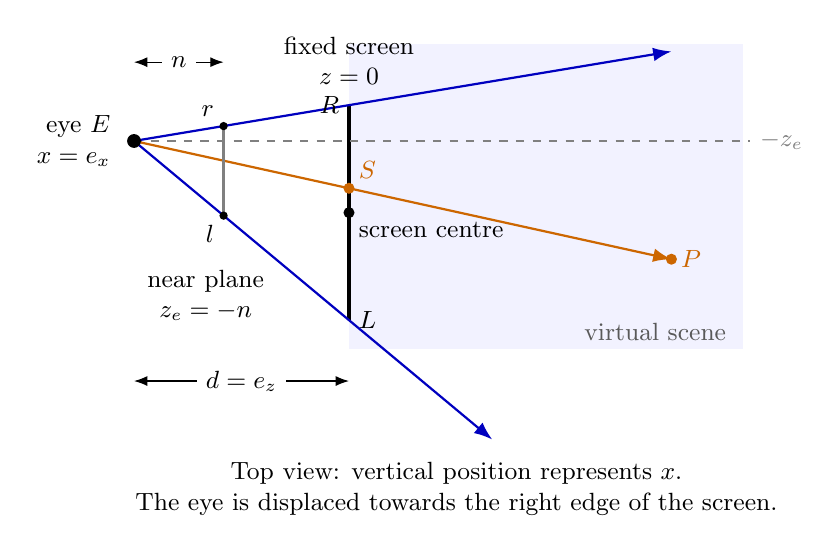
\begin{tikzpicture}[x=.91cm,y=.91cm,>=Latex,font=\small]
\fill[blue!5] (3,-1.9) rectangle (8.5,2.35);
\node[anchor=north east,text=black!65] at (8.4,-1.4) {virtual scene};
\draw[very thick] (3,-1.5)--(3,1.5);
\node[above,align=center] at (3,1.65) {fixed screen\\$z=0$};
\draw[dashed,gray] (0,1)--(8.6,1) node[right] {$-z_e$};
\draw[blue!75!black,thick,->] (0,1)--(7.5,2.25);
\draw[blue!75!black,thick,->] (0,1)--(5,-3.167);
\draw[orange!80!black,thick,->] (0,1)--(7.5,-.65);
\fill (0,1) circle (2.5pt) node[left=5pt,align=right] {eye $E$\\$x=e_x$};
\fill (3,0) circle (2pt) node[below right] {screen centre};
\fill[orange!80!black] (3,.34) circle (2pt) node[above right] {$S$};
\fill[orange!80!black] (7.5,-.65) circle (2pt) node[right] {$P$};
\node[left] at (3,1.5) {$R$};\node[right] at (3,-1.5) {$L$};
\draw[thick,gray] (1.25,-.05)--(1.25,1.208);
\fill (1.25,1.208) circle (1.5pt) node[above left] {$r$};
\fill (1.25,-.042) circle (1.5pt) node[below left] {$l$};
\node[align=center] at (1,-1.15) {near plane\\$z_e=-n$};
\draw[<->] (0,2.1)--(1.25,2.1) node[midway,fill=white] {$n$};
\draw[<->] (0,-2.35)--(3,-2.35) node[midway,fill=white] {$d=e_z$};
\node[below,align=center] at (4.5,-3.35) {Top view: vertical position represents $x$.\\The eye is displaced towards the right edge of the screen.};
\end{tikzpicture}
\caption{Off-axis geometry. The near-plane interval $[l,r]$ is the scaled image of the fixed screen interval as seen from the eye. Distances to the two boundary rays are unequal.}
\label{fig:offaxis}
\end{figure}

Applying similar triangles independently to the four screen edges gives
\begin{equation}\label{eq:offbounds}
\boxed{\quad l=n\frac{L-e_x}{e_z},\quad r=n\frac{R-e_x}{e_z},\quad
b=n\frac{B-e_y}{e_z},\quad t=n\frac{T-e_y}{e_z}.\quad}
\end{equation}
These bounds are signed coordinates, not necessarily negative on the left or positive on the right. The eye can lie outside the perpendicular footprint of the screen while the construction remains valid, provided $e_z>0$.

\newpage
\subsection{Derivation of the asymmetric matrix}
For a point $(x_e,y_e,z_e)$ in eye coordinates, the ray intersects the near plane at
\begin{equation}
x_n=-n\frac{x_e}{z_e},\qquad y_n=-n\frac{y_e}{z_e}.
\end{equation}
Mapping $[l,r]$ and $[b,t]$ to $[-1,1]$ then gives
\begin{align}
x_{\ndc}&=\frac{2x_n-(r+l)}{r-l}
=-\frac{2n}{r-l}\frac{x_e}{z_e}-\frac{r+l}{r-l},\\
y_{\ndc}&=\frac{2y_n-(t+b)}{t-b}
=-\frac{2n}{t-b}\frac{y_e}{z_e}-\frac{t+b}{t-b}.
\end{align}
Choosing $w_{\clip}=-z_e$ shows that the corresponding homogeneous numerators are
\begin{equation}
x_{\clip}=\frac{2n}{r-l}x_e+\frac{r+l}{r-l}z_e,\qquad
y_{\clip}=\frac{2n}{t-b}y_e+\frac{t+b}{t-b}z_e.
\end{equation}
The depth derivation is unchanged, giving the off-axis perspective matrix
\begin{equation}\label{eq:offmatrix}
\boxed{P_{\mathrm{off}}=\begin{pmatrix}
\frac{2n}{r-l}&0&\frac{r+l}{r-l}&0\\
0&\frac{2n}{t-b}&\frac{t+b}{t-b}&0\\
0&0&-\frac{f+n}{f-n}&-\frac{2fn}{f-n}\\
0&0&-1&0
\end{pmatrix}.}
\end{equation}
The positive signs in the third column are required: division by $w_{\clip}=-z_e$ produces the negative constant offsets in the normalised coordinates. The complete transformation is
\begin{equation}
\vect p_{\clip}=P_{\mathrm{off}}V\widetilde{\vect p}_w,
\qquad\text{or}\qquad
\vect p_{\clip}=P_{\mathrm{off}}VM\widetilde{\vect p}_{\mathrm{model}}
\end{equation}
when a model-to-world matrix $M$ is also needed. An eye-tracked renderer updates both $V$ and the bounds in~\eqref{eq:offbounds} from the eye position, while keeping the physical screen geometry fixed.

Several checks follow directly from the construction. A ray through the left screen edge has $x_e/z_e=-l/n$, so substitution gives $x_{\ndc}=-1$; the right, bottom and top edges similarly map to $1,-1,1$. The near and far planes map to depths $-1$ and $1$. When $e_x=(L+R)/2$ and $e_y=(B+T)/2$, the sums $r+l$ and $t+b$ vanish, reducing~\eqref{eq:offmatrix} to the centred matrix~\eqref{eq:symmetric}.

The screen intersection can also be verified directly in world coordinates. For a point $P=(X,Y,Z)$, the line $E+\lambda(P-E)$ meets $z=0$ when
\begin{equation}
\lambda=\frac{e_z}{e_z-Z},\qquad
X_s=e_x+\lambda(X-e_x),\qquad
Y_s=e_y+\lambda(Y-e_y).
\end{equation}
Normalising $(X_s,Y_s)$ using the fixed screen bounds gives exactly the same image coordinates as $P_{\mathrm{off}}V$. In particular, points already on the screen ($Z=0$) remain at their screen positions as the eye moves. Points away from the screen move in the image, producing motion parallax.

\newpage
\subsection{A screen with arbitrary position and orientation}
The same derivation applies when the screen is not aligned with the world axes. Let $A$ be its lower-left corner, $B_s$ its lower-right corner and $C$ its upper-left corner, as viewed from the eye. Assume a rectangular, planar screen and define
\begin{equation}
\vect u=\frac{B_s-A}{\|B_s-A\|},\qquad
\vect v=\frac{C-A}{\|C-A\|},\qquad
\vect k=\vect u\times\vect v.
\end{equation}
The vectors $\vect u$ and $\vect v$ point right and up on the screen; $\vect k$ points from the screen towards the viewer. For an eye position $E$, define
\begin{equation}
\vect a=A-E,\qquad \vect b=B_s-E,\qquad \vect c=C-E,\qquad
d=-\vect k^{\mathsf T}\vect a>0.
\end{equation}
An eye-centred, screen-aligned coordinate system is obtained using
\begin{equation}
V=\begin{pmatrix}
\vect u^{\mathsf T}&-\vect u^{\mathsf T}E\\
\vect v^{\mathsf T}&-\vect v^{\mathsf T}E\\
\vect k^{\mathsf T}&-\vect k^{\mathsf T}E\\
\vect 0^{\mathsf T}&1
\end{pmatrix}.
\end{equation}
In these coordinates, all screen corners lie in $z_e=-d$. Scaling their horizontal and vertical components onto the near plane gives
\begin{equation}
l=\frac{n}{d}\vect u^{\mathsf T}\vect a,\qquad
r=\frac{n}{d}\vect u^{\mathsf T}\vect b,\qquad
b=\frac{n}{d}\vect v^{\mathsf T}\vect a,\qquad
t=\frac{n}{d}\vect v^{\mathsf T}\vect c.
\end{equation}
Substituting these four quantities into~\eqref{eq:offmatrix} completes the construction without changing the projection formula. Eye coordinates, screen corners, and scene geometry must be expressed in a common coordinate frame and consistent units before applying it.

For example, take a screen $0.60\,\mathrm m$ wide and $0.34\,\mathrm m$ high, centred at the world origin in $z=0$, with the eye at $(0.10,0.04,0.60)\,\mathrm m$. For $n=0.10\,\mathrm m$ and $f=10\,\mathrm m$, equation~\eqref{eq:offbounds} gives
\begin{equation}
(l,r,b,t)=(-0.066667,\ 0.033333,\ -0.035000,\ 0.021667)\,\mathrm m,
\end{equation}
and, to six decimal places,
\begin{equation}
P_{\mathrm{off}}\approx\begin{pmatrix}
2&0&-0.333333&0\\
0&3.529412&-0.235294&0\\
0&0&-1.020202&-0.202020\\
0&0&-1&0
\end{pmatrix}.
\end{equation}
The world-space screen centre transforms to $(-0.10,-0.04,-0.60)$ in eye coordinates and then to $x_{\ndc}=y_{\ndc}=0$. This illustrates why the asymmetric terms are needed: they keep the physical screen's coordinate system fixed despite the displaced eye.
\end{document}
